\begin{frame}
  \frametitle{编程思想}
  \begin{itemize}
    \item 粗略的说,程序=数据结构+算法:
      \begin{itemize}
        \item 数据结构:数据是如何在计算机中存储的
        \item 算法:如何操作数据结构
      \end{itemize}
    \item “编程思想”要\underline{解决的问题}:在软件编程中,如何将真实世界中的复杂事物刻画映射为计算机程序中可编程的数据结构和算法
    \item 目前最为常用的两类编程思想:\underline{面向过程}和\underline{面向对象}
  \end{itemize}
\end{frame}

\begin{frame}
  \frametitle{面向过程编程}
  \begin{itemize}
    \item 面向过程的程序设计把计算机程序视为一系列的命令集合,即一组函数的顺序执行。“过程”就是函数!
    \item “面向过程编程”的\underline{基本思路}:把事物设计为函数,然后把大块函数通过切割成小块函数来降低系统的复杂度。
    \item 程序的设计、编写和运行,本质上都是采用了一种线性的思维
    \item 大家以前学习的C语言就是一门最常见的“面向过程”的编程语言。C语言的入口为主函数\texttt{main},在该函数中调用其它用户设计实现的程序子函数
  \end{itemize}
  \center{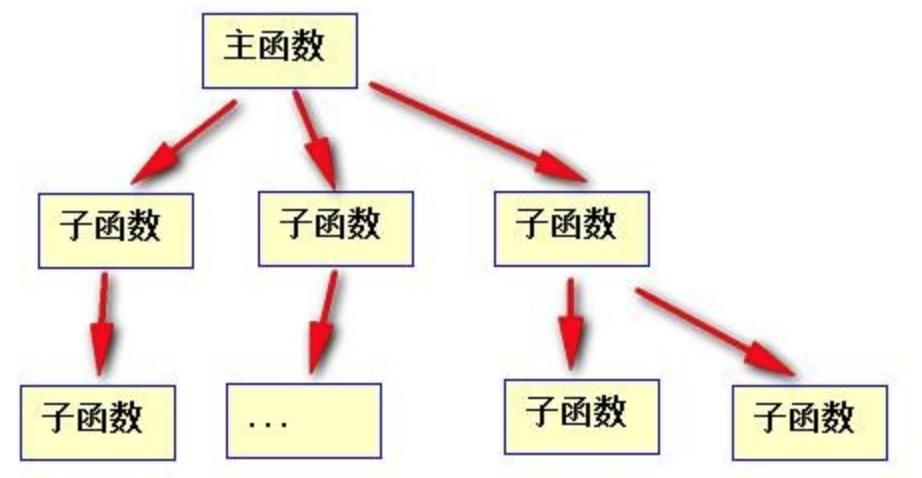
\includegraphics[width=\textwidth/2]{figures/pop}}
\end{frame}

\begin{frame}
  \frametitle{面向对象编程}

    “面向对象编程”(OOP,Object Oriented Programming)的\underline{基本思路}:
    
    将真实世界中的复杂事物抽象、提取、归纳为“对象”
%    \item 把一组数据结构和处理它们的方法组成对象(object),把相同行为的对象归纳为类(class),通过类的封装(encapsulation)隐藏内部细节,通过继承(inheritance)实现类的特化(specialization)/泛化(generalization),通过多态(polymorphism)实现基于对象类型的动态分派(dynamic dispatch)。
  \\
  \\
  举例——历史学家要编写史书,主要有两种形式:
      \begin{itemize}
        \item 纪传史:以人物为中心编写,可以类比为“面向对象”
        \item 编年史:按照事件发生的事件顺序编写,可以类比为“面向过程”
      \end{itemize}

\end{frame}

\begin{frame}
  \frametitle{对象(object)}
  \begin{itemize}
    \item OOP把对象作为程序的基本单元,一个对象包含了:
      \begin{itemize}
        \item 属性:即数据,描述了“该对象有什么数据”
        \item 方法:即操作数据的函数,描述了“该对象能干什么”
      \end{itemize}
    \item 对象=属性(attribute)+方法(method)
    \item 例子一:将“人”这个概念抽象为“对象”
      \begin{itemize}
        \item 属性:姓名、年龄、性别 ...
        \item 方法:吃饭、睡觉、走路 ...
      \end{itemize}
    \item 例子二:将“汽车”这个概念抽象为“对象”
      \begin{itemize}
        \item 属性:发动机、底盘、车身、油箱 ...
        \item 方法:启动、行车、刹车、加油 ...
      \end{itemize}
  \end{itemize}
\end{frame}

\begin{frame}[t]
  \frametitle{面向过程和面向对象在解决问题思路上的差别}
  \center{\textbf{问题:人把大象装冰箱}}
  \vspace{1pt}
  \begin{columns}[t]
    \column{0.4\textwidth}
      \center{\textbf{面向过程的思路}}
      
      \vspace{1pt}
      程序入口主函数:
      \begin{enumerate}
        \item 函数一:打开冰箱
        \item 函数二:把大象塞进去
        \item 函数三:关冰箱门
      \end{enumerate}
    \column{0.6\textwidth}
      \center{\textbf{面向对象的思路}}
      
      \vspace{1pt}
      \underline{设计对象}(只定义了“方法”):
      \begin{itemize}
        \item 人:操作(冰箱),操作(大象)
        \item 大象:进入()
        \item 冰箱:开门(),关门()
      \end{itemize}
       程序入口主函数:
       \begin{enumerate}
         \item 人.操作(冰箱):冰箱.开门()
         \item 人.操作(大象):大象.进入()
         \item 人.操作(冰箱):冰箱.关门()
       \end{enumerate}
  \end{columns}
\end{frame}

\begin{frame}
  \frametitle{类(class)}
  \begin{itemize}
    \item “类”是对一类事物的总结,可以把“类”理解为:对大量对象共性的抽象,是对象的模板。“类”中定义了这一类对象的共有属性和共有方法
    \item “类”具有属性(也称成员变量),它是对象的属性状态的抽象,用数据结构来描述类的属性,人类有姓名、年龄、性别等属性
    \item “类”具有操作(也称方法),它是对象的操作行为的抽象,用操作名和实现该操作的方法来描述,人有吃()、说话()、学习()等方法
    \item “类”的具体化就是对象,也可以说类的实例是对象。如有“人”这个类,统称人类;对象则是具体的某个人,如张三、李四
  \end{itemize}

\end{frame}

\begin{frame}
  \frametitle{类的举例}
  \center{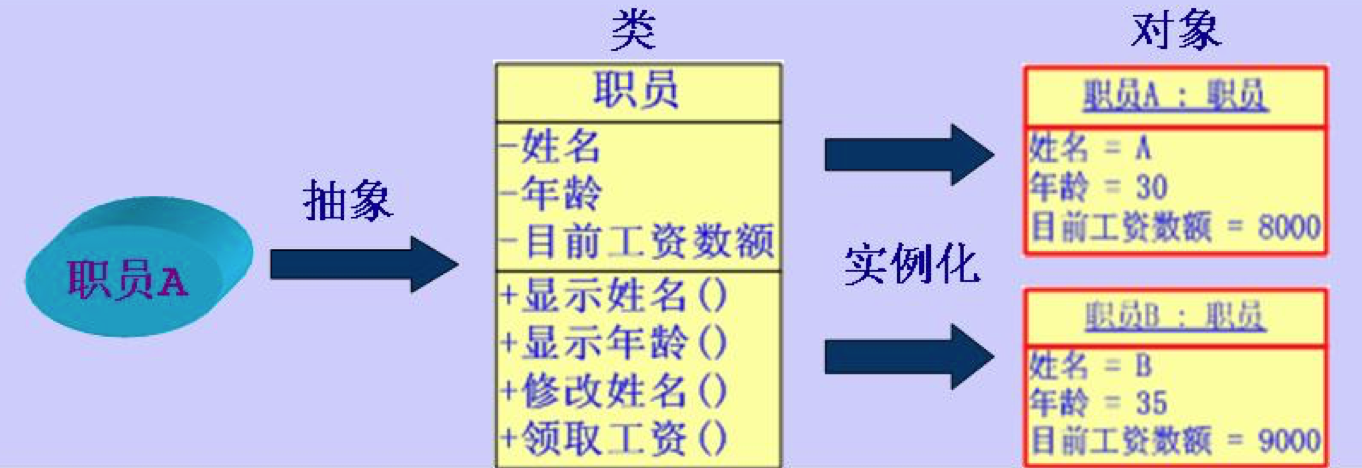
\includegraphics[width=0.8\textwidth]{figures/class_object1}}
  \center{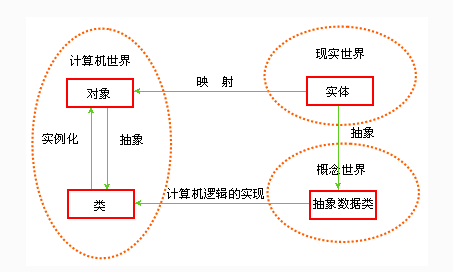
\includegraphics[width=0.7\textwidth]{figures/class_object2}}
\end{frame}

\begin{frame}
  \frametitle{Java中的面向对象编程}
  \begin{itemize}
    \item Java是一门OOP语言\footnote{严格来说,Java只是一门较为纯粹的OOP语言,仍然有一些不属于OOP的元素},在Java中对象是第一公民,程序的设计和编写都是围绕着各种对象展开的
    \item 和Java相对的,C语言这种面相过程的编程语言,函数往往是第一公民
    \item 面向对象的好处:易维护、易复用、易扩展
    \item 在Java中,定义在类中的函数一般称为“方法”
  \end{itemize}
\end{frame}
